% Figure 2. What the student sees versus what the model receives. Compile: pdflatex fig_channel.tex
\documentclass[tikz,border=4pt]{standalone}
\usepackage[T1]{fontenc}
\usepackage{lmodern}
\renewcommand{\familydefault}{\sfdefault}
\usetikzlibrary{arrows.meta,positioning,calc,fit}
\definecolor{OX}{HTML}{C0392B}
\definecolor{RED}{HTML}{E8765C}
\definecolor{AMBER}{HTML}{E4A857}
\definecolor{CHOC}{HTML}{A9705A}
\definecolor{TAUPE}{HTML}{8C776C}
\begin{document}
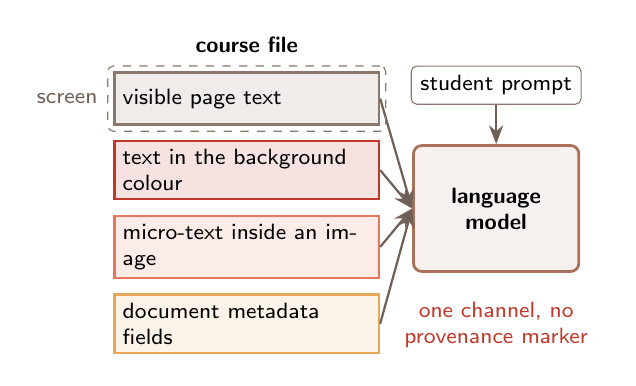
\begin{tikzpicture}[
  font=\footnotesize,
  layer/.style={draw=#1,fill=#1!14,line width=0.8pt,minimum width=3.3cm,
    minimum height=0.66cm,align=left,text width=3.15cm,inner sep=3pt},
  flow/.style={-{Stealth[length=2.4mm]},line width=0.8pt},
]
\node[layer=TAUPE] (v)  {visible page text};
\node[layer=OX,below=0.18cm of v]  (w)  {text in the background colour};
\node[layer=RED,below=0.18cm of w]  (i)  {micro-text inside an image};
\node[layer=AMBER,below=0.18cm of i] (m) {document metadata fields};
\node[font=\footnotesize\bfseries,above=0.12cm of v] {course file};

\node[draw=CHOC,line width=1pt,fill=CHOC!10,rounded corners=3pt,minimum width=2.1cm,
  minimum height=1.6cm,align=center,right=2.1cm of $(w)!0.5!(i)$] (llm)
  {\textbf{language}\\\textbf{model}};
\node[draw=TAUPE,rounded corners=2pt,fill=white,align=center,minimum width=2.1cm,
  above=0.5cm of llm] (prompt) {student prompt};

\foreach \n in {v,w,i,m}{\draw[flow,color=TAUPE!80!black] (\n.east) -- (llm.west);}
\draw[flow,color=TAUPE!80!black] (prompt) -- (llm);

\node[draw=TAUPE,dashed,rounded corners=2pt,fit=(v),inner sep=2pt,
  label={[font=\footnotesize,text=TAUPE!80!black,anchor=east]west:screen}] {};
\node[font=\footnotesize,text=OX,align=center,below=0.25cm of llm,text width=2.6cm]
  {one channel, no\\ provenance marker};
\end{tikzpicture}
\end{document}
